\documentclass[sigconf]{acmart}
\usepackage{balance}

\fancyhf{} % Remove fancy page headers 
\fancyfoot[C]{\thepage}

\setcopyright{none} % No copyright notice required for submissions
\acmConference[Anonymous Submission to ACM CCS 2017]{First ACM CCS Workshop on IoT Security & Privacy}{Due 11 August 2017}{Dallas, Texas}
\acmYear{2017}

\settopmatter{printacmref=false, printccs=true, printfolios=true} % We want page numbers on submissions

%%\ccsPaper{9999} % TODO: replace with your paper number once obtained

\begin{document}
\title{Plaintext Data Transmissions in Medical IoT Systems} % TODO: replace with
% your title
\author{Daniel Wood}
\affiliation{\institution{Princeton University}}
\email{dewood@princeton.edu}
\author{Noah Apthorpe}
\affiliation{\institution{Princeton University}}
\email{apthorpe@princeton.edu}
\author{Nick Feamster}
\affiliation{\institution{Princeton University}}
\email{feamster@princeton.edu}

% The default list of authors is too long for headers}
\renewcommand{\shortauthors}{D. Wood et al.}


\begin{abstract} 
This paper introduces a method of deep packet inspection to
capture transmitted data from medical IoT devices and analyze plaintext and
metadata for information that reveals a user's medical conditions and
behavior. After analyzing multiple devices, we present concerning results of a
smart medical device that leaks plaintext data. The research follows a three-
step approach involving data collection, deep packet inspection, and data
representation. We present this capability for IoT device analysis
through a
user-friendly interface for consumers to monitor and visualize vulnerabilities
of IoT devices in their home.  
\end{abstract}

\keywords{Internet of Things, privacy, medical devices, patient health information, encryption, deep packet inspection}

\maketitle

\section{Introduction}

According to the Federal Trade Commission, ``The Internet of Things (``IoT'') refers to the ability of everyday objects to connect to the Internet and to send and receive data'' ~\cite{ftc}. This definition includes a variety of internet-connected medical devices increasingly deployed in homes and hospital environments. These devices are designed to record patient data and integrate measurements into electronic health records. User data collected by medical IoT devices is especially privacy sensitive, and device manufacturers may be legally obligated to handle such data in accordance with the Health Insurance Portability and Accountability Act of 1996 (HIPAA). 

The Security and Privacy rules of HIPAA require covered entities to maintain appropriate
administrative, technical, and physical safeguards for protecting electronic patient health information~(e-PHI)~\cite{securityHIPAArule, privacyHIPAArule}. HIPAA defines e-PHI as individually identifiable health information, including:
\begin{enumerate}
  \item an individual's past, present or future physical or mental health or condition
  \item the provision of health care to an individual
  \item the past, present, or future payment for the provision of health care to an individual
  \item common identifiers, e.g., name, address, birth date, and  Social Security Number
\end{enumerate}
Entities that collect e-PHI are required to:
\begin{enumerate}
  \item Ensure the confidentiality, integrity, and availability of all e-PHI they create, receive, maintain, or transmit
  \item Identify and protect against reasonably anticipated threats to the security or integrity of the information
  \item Protect against reasonably anticipated, impermissible uses or disclosures
\end{enumerate}
\noindent
Many medical IoT devices enable users to track their personal health via their
smartphones and have the potential to leak e-PHI.  Encryption is the most
obvious determinant of confidentiality in medical IoT device communications.
Packets of data sent in the clear can be trivially intercepted by adversaries
and network observers. Even if plaintext data is compressed, it is still
trivial to recover the original content by recovering the compressed message
and attempting decompression using a limited number of widely used compression
algorithms. Transmitting application data in the clear is a severe (and
seemingly obvious) design flaw, and yet it is prevalent among IoT
devices~\cite{tinker}.

Even when medical IoT devices encrypt data transmitted to the cloud, a network
observer could scrutinize metadata to obtain information about a user.
Several recent studies have demonstrated that IoT device traffic analysis can
reveal user behavior  from correlations between device network activity and
user interactions~\cite{apthorpeIoT}.

This paper examines whether in the course of regular behavior, today's
commercially available smart medical devices properly protect all individually
identifiable health information as dictated by HIPAA.  We evaluate a suite of
medical IoT devices, including: (1)~the Withings Smart Blood Pressure Monitor,
(2)~Withings Smart Scale, (3)~iHealth Ease Wireless Blood Pressure Monitor, and (4)~1byOne
Digital Smart Wireless Scale, all of which are popular and readily available
on Amazon. We record and analyze network traffic from these devices and
attempt to identify plaintext health information and/or metadata that would
allow an adversary to infer e-PHI from encrypted communications.

We present two main findings. First, we find that multiple devices that were
tested send information related to their users' heath in plaintext. This
result is concerning given our relatively small sample of devices, and
indicates that plaintext transmission of heath information may be a widespread
privacy vulnerability across the market of IoT medical devices. Even more
worrisome, we found plaintext health information in communications from
devices that use SSL/TLS transport layer encryption. This health information
was sent in cookies, URLs, and occasional unencrypted connections---all
indicative of poor development practices by device manufacturers.

Secondly, even the devices that consistently encrypt health information have privacy
vulnerabilities. Network observers and adversaries can see
traffic from these devices as being generated from specific IP addresses. By
examining network traffic from an access point, it is possible to isolate
traffic originating from a fixed set of IP addresses and subsequently mine the
associated metadata for sensitive medical information. Although in some home and
hospital settings, individual IP addresses may be shielded by a NAT, the rise
of IPv6 and devices tethered to cell phones leave many devices directly exposed
and individually identifiable.

Though patients and doctors expect their e-PHI to be properly protected, one
of the major problems with commercially available IoT devices on the market is
the user's lack of visibility in terms of how their data is handled. This
paper presents a simple and intuitive user interface for IoT device users to
monitor and visualize the data that their medical IoT devices transmit to the
Internet. As traffic data from a suite of connected devices is captured on a
local Wi-Fi access point, we mine the traffic for potentially revealing
electronic personal health information that has been transmitted in the clear.
The user interface lists each device connected to the access point, warning
the user of potential plaintext leakages associated with each device (Figure
1). The goal was to make the interface universally intelligible so that
average users with no comprehension of packets, encryption, or networks would
be able to monitor how each device protected their e-PHI.

We recently presented our findings to members of congress, including Senator
Edward Markey~(MA) and Congressman Joe Kennedy~(MA), to raise awareness of the
potential vulnerabilites in IoT devices and of the lack of security or privacy
standardization among IoT device manufacturers. As a featured
participant in the Coalition for National Science Funding's 2017 Capital Hill Exhibition,
we addressed the need for increased consumer visibility into the data that their
IoT devices are sending across the Internet through a unified web-based dashboard~\cite{cra}.
\begin{figure}[t]
  \centering
    \fbox{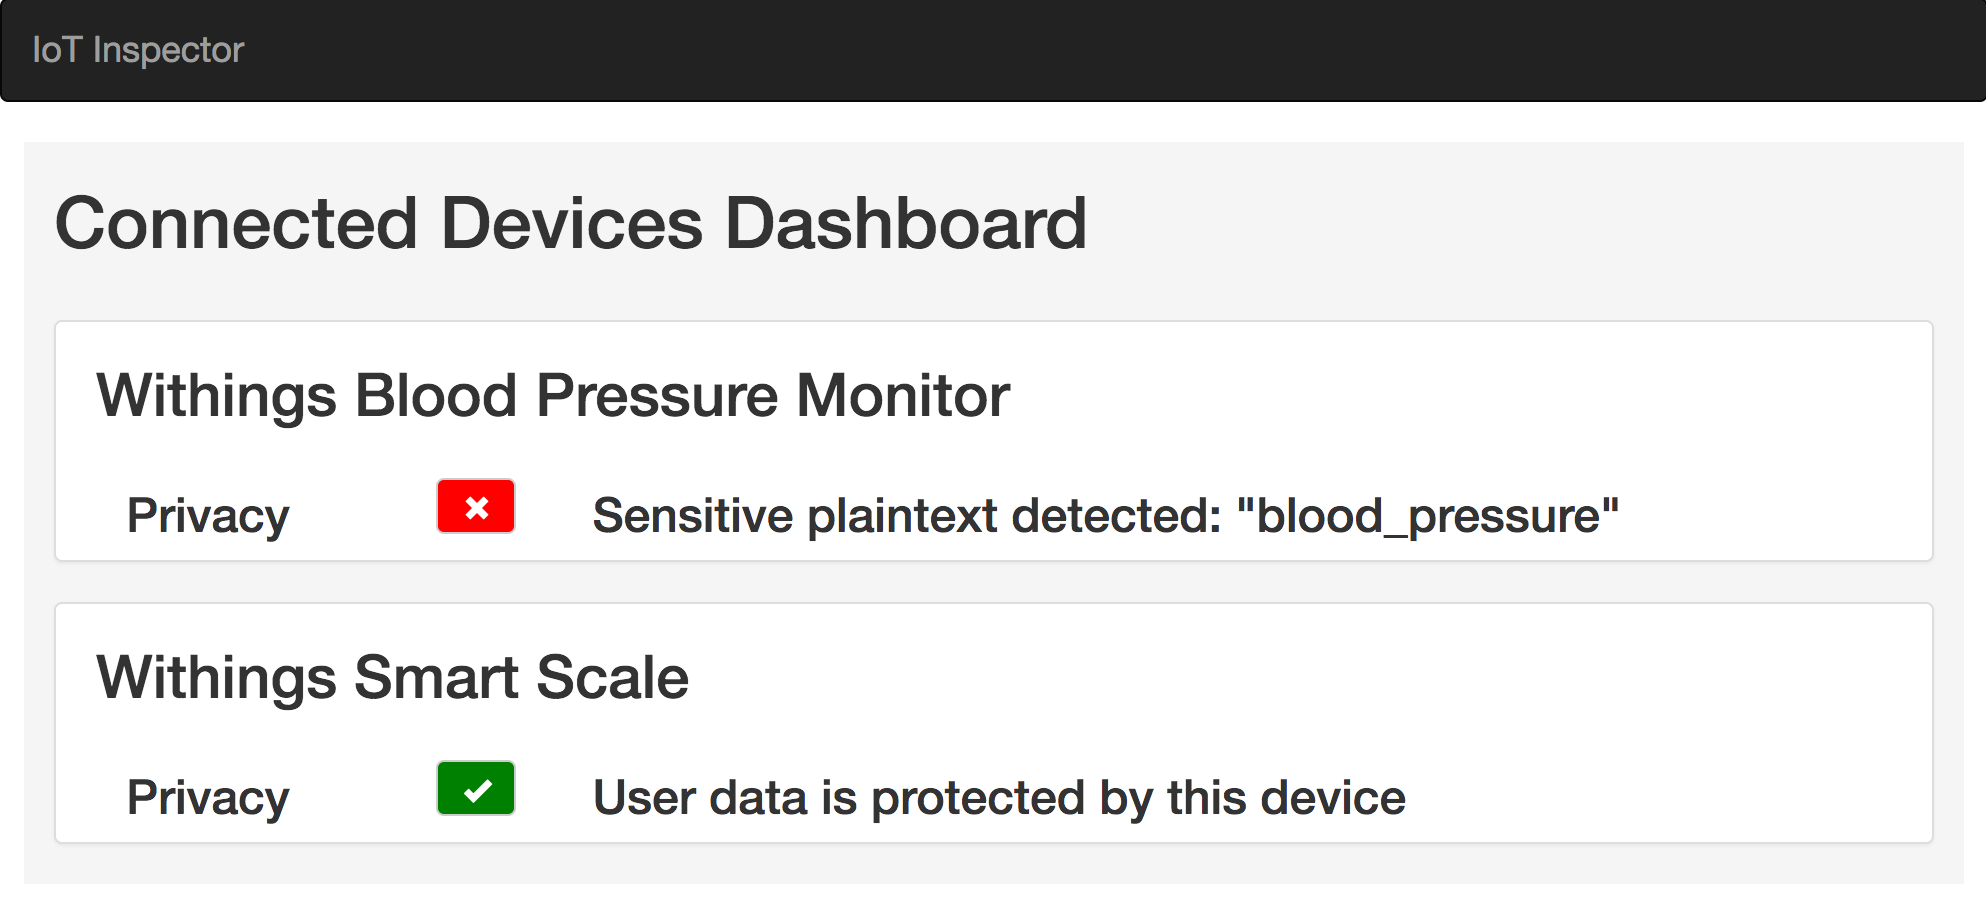
\includegraphics[width=\linewidth]{dashboard}}
  \caption{User interface displays connected devices in the home and privacy status.}
  \label{fig:dashboard}
\end{figure}

\section{Related Work}

Classifying network traffic as
encrypted or plaintext can be challenging. Cha outlines the following
method to determining encrypted versus unencrypted traffic~\cite{chaMachineLearning}:
\begin{enumerate}
  \item Separate each packet's header (non-encrypted) from its payload (potentially encrypted)
  \item Analyze randomness of payload using multiple tests, including Shannon Entropy, Chi-square, and arithmetic mean
  \item Use a training subset from plaintext protocols (HTTP, FTP, Telnet) and encrypted protocols (SSH, TLS) to determine a threshold entropy, above which indicates encrypted traffic
\end{enumerate}
\noindent
We use this approach as a baseline method for classifying traffic. A related
problem is distinguishing encrypted traffic from compressed plaintext traffic,
which is more difficult since both compressed and encrypted traffic exhibit
high orders of entropy. In this paper, we restrict our focus to distinguishing
uncompressed plaintext traffic from encrypted traffic.

Related research into the privacy implications of IoT systems has revealed
significant privacy vulnerabilities that adversaries with passive network
capabilities could exploit. However, most of the literature uses data
collected from generic home devices, not medical IoT devices. For example, Srinivasan et al. present a new privacy
leak in residential wireless ubiquitous computing systems: the Fingerprint and
Timing-based Snooping (FATS) attack~\cite{srinivasan2008fats}.
This attack allows a WiFi eavesdropper to
observe private activities in the home such as cooking, showering, toileting,
and sleeping by snooping on the wireless transmissions of sensors in a home
and leveraging tiered inference algorithms.

 Copos et al. present a scheme to infer when a home is occupied based on parsing
 packet capture files and log characteristics of the network traffic from a smart thermostat~\cite{coposIoT}.
More recently, Apthorpe et al. ~\cite{apthorpeIoT} observed that passive network observers, such as Internet service providers, could analyze IoT network traffic and infer user/device interactions even when device communications are encrypted. 
%By analyzing metadata from four smart home devices (a Sense sleep monitor, a Nest Cam Indoor security camera, a WeMo switch, and an Amazon Echo), Apthorpe measured the correlation between traffic rates and user interaction. He showed that 
%Even when IoT traffic is encrypted, information such as network patterns reveal potentially sensitive user information that third parties and adversaries would find valuable. 
This attack is especially concerning for personal medical devices. The repetitive nature of medical tests, such as daily blood sugar or blood pressure readings, generates clearly defined patterns of device activity and could reveal common medical conditions from network metadata alone. 

%Apthorpe introduces a three-step strategy that a passive network observer could use ``to identify devices in a smart home and infer user behavior.'' First, an adversary must separate the device traffic into packet streams. Second, an adversary must label streams by type of device by performing reverse DNS lookups to ``pair service IP's with device identifying domain names.'' Only once each device's traffic has been isolated, will an adversary be able to examine a device's traffic rate to infer user behavior of the device. 

Dimitrov notes that
% ``The Internet of Things (IoT) is a network of physical devices and other items, embedded with electronics, software, sensors, and network connectivity, which enables these objects to collect and exchange data.''$^2$
the proliferation of the medical Internet of Things will revolutionize digital healthcare
by enabling doctors and hospital systems to streamline workflows, increase productivity,
and provide higher data-backed quality of care~\cite{dimitrovIoT}. The research
highlights five key capabilities that leading platforms must enable: (1) Simple
connectivity, (2) Easy device management, (3) Information ingestion, (4) Informative analytics, and (5) reduced risk. In this work, we attempt to improve device management and informative analytics by creating a dashboard that analyzes real-time traffic flows from smart medical devices and informs the user of potential privacy vulnerabilities.

\section{Device Evaluation Methods}

We analyzed medical IoT device network traffic for privacy vulnerabilities using a three phase process:

\begin{enumerate}
  \item Data collection: where we convert a Raspberry Pi into a Wi-Fi access point and collect traffic from a suite of connected IoT devices
  \item Plaintext identification: where we search captured traffic for plaintext application data revealing patient information
  \item Metadata analysis: where we examine second order information such as device activity to infer user behavior
\end{enumerate}

\subsection{Data Collection}

We created an isolated test environment where we could connect various medical IoT devices to a network and capture live traffic. We configured a Raspberry Pi 3 as a Wi-Fi access point (AP) and programmed it to record traffic to and from connected Wi-Fi stations (Figure~\ref{fig:data-collection}). The open source code can be examined at $github.com/danielwood95/IoTSecurityHub$.  Creating an isolated test environment was necessary because it enabled us to easily separate traffic by device and filter out extraneous traffic on the network.   We chose four mIoT devices to inspect:

\begin{enumerate}
  \item Withings Wireless Blood Pressure Monitor
  \item Withings Body Composition Wi-Fi Scale
  \item 1byOne Digital Smart Wireless Body Fat Scale
  \item iHealth Ease Wireless Blood Pressure Monitor
\end{enumerate}

\begin{figure}
  \centering
    \fbox{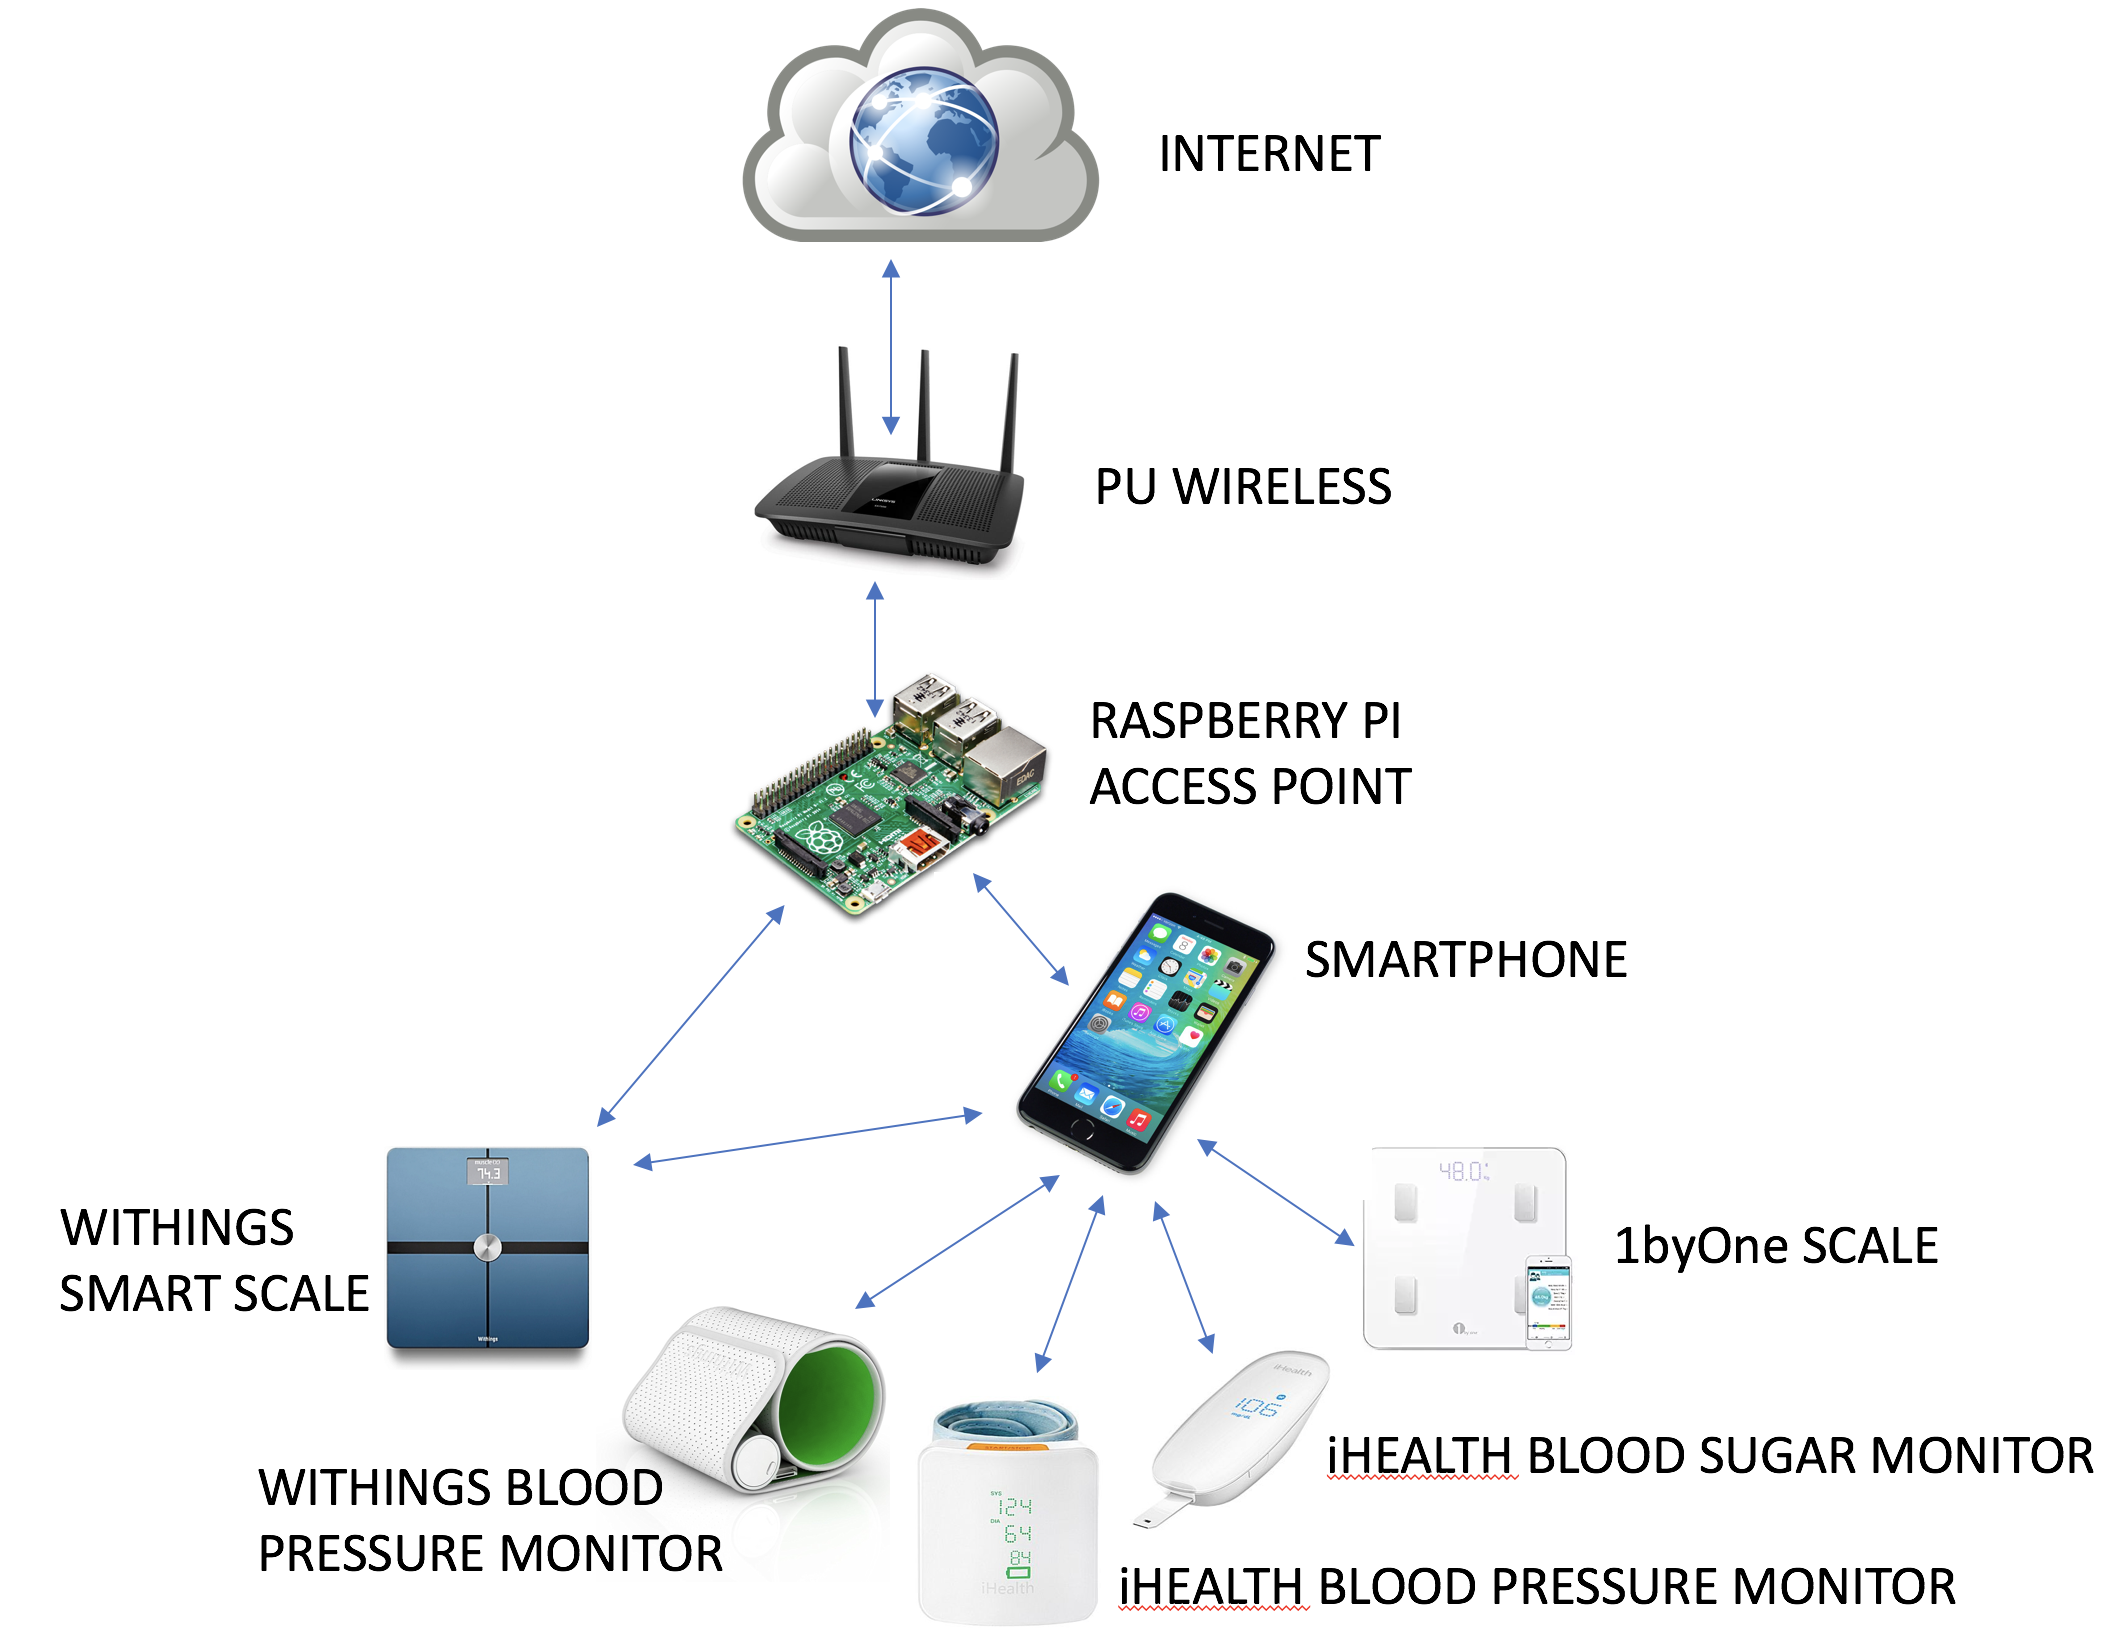
\includegraphics[width=\linewidth]{network}}
  \caption{Data collection environment and connection patterns between devices and infrastructure components.}
  \label{fig:data-collection}
\end{figure}

We connected the Wi-Fi-enabled directly to the Raspberry Pi AP and the Bluetooth-enabled devices to a smartphone connected to the AP.
%These devices are different from those analyzed in studies such as \cite{apthorpeIoT} because theirshort-lived (i.e. only transmit data when in use for measuring blood pressure, weight, blood sugar, etc.). This provides intuitive frequency metadata and enables passive network observers to easily determine when a patient is using the device and how often. On the other hand, long-lived devices such as Amazon Echo or Nest are constantly transmitting data, though the number of packets sent increases substantially when the device is being actively used. 
We purposefully chose two smart scales and two blood pressure monitors so that we could compare the way in which different device manufacturers transmit application data and determine which company had better security or privacy practices, if any. 

We used Wireshark to capture all Ethernet traffic traversing the access point, divided these data using MAC addresses into streams of packets corresponding to each IoT device, and saved the packets in PCAP files for offline analysis. 
 When generating the dataset, we captured as many use cases of each device as possible, including user registration and sign-up, downloading patches and updates, vitals measurements, and health analytics. It is important not to ignore the use cases beyond general vitals measurement, because some of the most valuable information obtainable by an adversary would be a patch because it could reveal information about the way the embedded system in the device is designed. 

\subsection{Plaintext Identification}

We next analyzed captured packet streams from our medical IoT devices for unencrypted health information. We started by separating the packets by protocol, focusing mainly on HTTP and TCP packets and ignoring packets sent with SSL or TLS, as those are encrypted. Next we separated the payload, which contains application data, from the header of each packet for further analysis. Even though HTTP and TCP are unencrypted, it was still necessary to eliminate payloads containing encrypted application-level data so we could concentrate our analysis on unencrypted application-level data. We experimented with three different schemes for this classification: naive ASCII approach, Shannon entropy test, and chi squared test. The latter two are approaches tested by Cha et al. ~\cite{chaMachineLearning}.

\subsubsection{Naive ASCII approach}
%The first approach used to determine whether a packet was plaintext or encrypted was the naive ASCII approach. 
If all the characters in the payload are contained within the 128 character ASCII set, we anticipated that a packet would be unencrypted, since encrypted packets would need to contain characters from the extended ASCII set. While the naive ASCII approach does weed out encrypted packets, it does not identify all unencrypted packets, many of which contain characters from the extended ASCII set in addition to the printable characters. 

\subsubsection{Shannon Entropy Test}
%The next approach used determine whether or not a packet was encrypted was the Shannon Entropy Test. 
The Shannon Entropy Test calculates the entropy of each payload string, which is a quantitative measure of the variability in the frequency of the different possible characters. While random (or in this case, encrypted) strings have very high entropy, unencrypted plaintext and English strings exhibit fairly low entropy. To calculate the Shannon Entropy of a string, let $X$ be a random variable that takes on possible values $x_1$, $x_2$, ..., $x_n$. $p(x_i)$ is the probability that $X = x_i$:
$$H(X) = - \sum_{i = 1}^{n} p(x_i) log p(x_i)$$
A packet's payload is presumed to be unencrypted if its Shannon entropy value is lower than a threshold parameter. For our analysis, we used a relatively high threshold parameter of $7.5$, so as not to discard some unencrypted payloads with high entropy (at the cost of misidentifying a small number of encrypted payloads with low entropy).

\subsubsection{Chi-Squared Test}
Lastly, the Chi-Squared test compares the frequency of each character with its expected value from a uniform distribution. The value $\chi^2$ is calculated according to the formula:
$$\chi^2 = \sum_{i=1}^{n} \frac{(o_i-e_i)^2}{e_i}$$
The more a set of frequencies deviates from its expected values, the higher the value of $\chi^2$, and if the observed frequencies equal the expected frequencies then $\chi^2$ is 0. Therefore, English plaintext is expected to have a much higher deviation of character frequencies from the expected frequency (a uniformly random distribution). By setting the threshold value $\chi^2 = 1000$, we were able to effectively weed out the unencrypted payloads from those that were encrypted. 

\subsubsection{Method Comparison}

To determine which of the three methods (naive ASCII, Shannon Entropy, or Chi-Squared)
yielded the most accurate classification of unencrypted packets, we ran a comparative analysis with five PCAP files with over 225,000 packets (Figure~\ref{fig:method-comp}). Out of the three methods, the naive ASCII approach was the most selective. It had a 0 percent false positive rate, but missed nearly all of the unencrypted packets, because many of the payloads contained some number extended ASCII characters. 

In contrast, the Shannon Entropy approach cast a much wider net, tagging a much larger share of packets as being unencrypted, though this approach suffered from a high false positive rate. Lowering the threshold entropy value did not significantly increase the accuracy of the approach, as fewer true unencrypted packets were identified as the threshold entropy value decreased. 

We found the most accurate encryption classification approach to be the Chi-Squared
test, due to its low false positive rate and identification of non-random string patterns within the packet payloads we tested. The Chi-Squared test exhibited a false positive rate of approximately 3.5\%, while still identifying nearly all the other unencrypted payloads as the naive ASCII and Shannon entropy approaches.


\begin{figure}
  \begin{center}
    \begin{tabular}{c|c|c} 
    \textbf{Approach} & \textbf{Precision} & \textbf{\% packets plaintext}\\ [0.5ex] 
    \hline
    Naive ASCII & $1$ & $0.5$ \\ 
    Shannon Entropy &  $0.26$ & $16.2$ \\
    Chi Square & $.97$ & $4.9$ \\
    \end{tabular}
    \caption{Comparison of plaintext detection approaches on 225,000 packet payloads from the devices studied. The precision metric indicates the probability that a particular approach correctly identifies a payload as plaintext. Column 3 indicates what percent of total packets were identified as plaintext. Less selective approaches identify more plaintext packets, but also result in higher false positive rates.}
    \label{fig:method-comp}
  \end{center}
\end{figure}

\subsubsection{Dictionary Analysis}
Once we were able to identify plaintext packets, we identified potentially sensitive personal medical/identifying information by searching each string in the plaintext payload in several dictionaries. We used three dictionaries: a list of the 100 most common medical terms/conditions from Barron's Medical Dictionary~\cite{barrons}, a list of the most popular first male and female names according to the U.S. Census Bureau~\cite{names}, and a list of the most common personal identifying information (i.e. passport number, license, name, address, etc.) according to the National Institute of Standards and Technology~\cite{nist}. 

\subsection{Metadata Analysis}

In cases when devices encrypted application-level data or utilized secure
protocols such as TLS or SSL, we were still able to infer rough user behavior
during traffic collection due to the fact that the devices studied are only
used to make periodic measurements and are not always on. For example, blood
sugar may be measured at regular intervals throughout the day (such as after a
meal) and smart scales might be used once every morning. Using Wireshark, we
were able to associate periods of device activity based on time stamps and
origin IP addresses, thereby keeping track of each device reading. In some
cases, we were able to determine what the behavior of the user during that
period of activity by examining the descriptions of the destination IP
addresses in Wireshark. For example, the Withings Smart Scale always
communicates with {\tt scalews.withings.net} when transmitting data
about a current measurement, making all outgoing traffic easily identifiable.

% \begin{figure}
%   \begin{center}
%     \begin{tabular}{c|c} 
%     \textbf{Dest IP} & \textbf{Description} \\ [0.5ex] 
%     \hline
%     $224.0.0.251$ & withings-aura-bridge.tcp.local \\ 
%     \hline
%     $172.24.1.1$ & scalews.withings.net \\
%     \hline
%     $172.24.1.1$ & maintws.withings.net \\
%     \hline
%     $172.24.1.1$ & static.withings.com \\ [1ex] 
%     \end{tabular}
%   \end{center}
%   \caption{Withings Smart Scale traffic destinations}
% \end{figure}

\section{Device Vulnerability Analysis}

We found a large variability in the methods each device used to send
application data through the network when registering users, sending patches
and updates, measuring vitals, or retrieving health analytics. All of the
devices used encryption and protocols such as TLS or SSH to send sensitive
first order information, such as the user's actual weight or blood sugar
levels. However, there were various degrees of leaking second order
information and metadata, scraped from sources such as HTTP GET requests,
packet header information, and device conversation IP tables. Of the devices
that we captured traffic for, the most secure implementation was the 1byOne
Digital Smart Wireless Body Fat Scale. This device not only used encrypted
protocols to deliver application data, but also masked names of packet
destinations, unlike the Withings devices.

\subsection{Blood Pressure Monitor: \\ Leaks in Plaintext}

The Withings Blood Pressure Monitor, out of the four devices monitored,
exhibited the most vulnerabilities concerning sensitive user information
during data transmission. We were able to capture enough sensitive second-
order data and metadata from a stream of traffic from the device in the course
of typical usage to determine that the user of the device was measuring his or
her blood pressure, and how frequently the user was taking these measurements as
well.

First of all, it is easy for a network observer to detect that a Withings IoT
device is in use, because the information sections of all queries and
responses to the Withings servers are titled with the brand of the device in
the URL. This would make it exceptionally easy for a network observer to track
all traffic originating from IP addresses querying an address such as
static.withings.com. Because of the limited capabilities of medical IoT
devices, as opposed to devices such as Amazon Echo, which can reach any
endpoint on the Internet, there is a limited number of endpoints that are
queried from each device, making device identification by a network observer
trivial.

Even more concerning, we observed that one of the signature characteristics of
the Withings Blood Pressure Monitor's traffic pattern was the fact that each
digital reading concluded with a GET request for a stock photo of a person
using the Withings Blood Pressure Monitor (Figure 4). This GET request is
certainly a cause for concern, as any adversary monitoring the traffic would
be able to immediately determine when a user has finished measuring his or her
blood pressure. This GET request was sent completely in the clear, and
furthermore, it is not even displayed on the user interface of the app to the
user of the device. It appears that there is no purpose of sending this image
upon the success of each blood pressure reading, except inadvertently
notifying network observers that the Withings Blood Pressure Monitor is in
use.

\begin{figure}[t]
  \centering
    \fbox{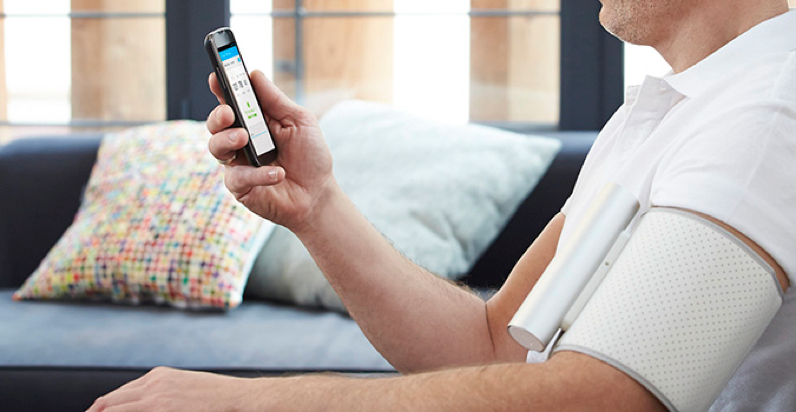
\includegraphics[scale=0.35]{bloodpressure}}
     \caption{Withings Blood Pressure Monitor sends image indicating device purpose in the clear.}
     \label{fig:bp-image}
\end{figure}

\begin{figure}[t]
  \centering
    \fbox{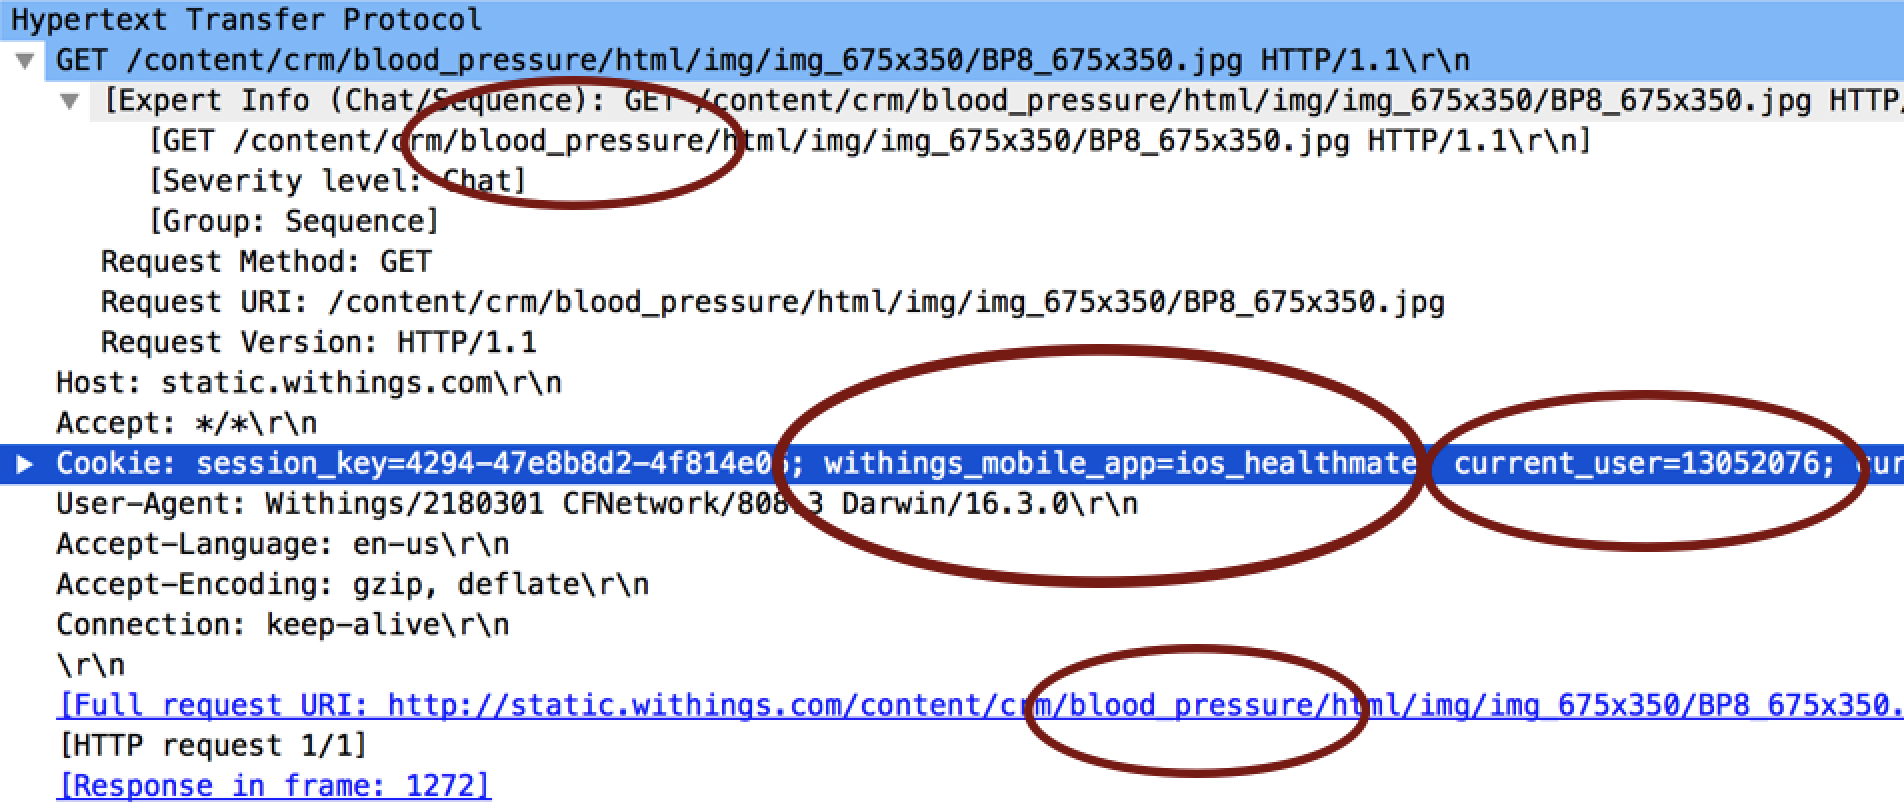
\includegraphics[width=\linewidth]{bloodpacket2}}
  \caption{HTTP packet sent by IoT blood pressure monitor reveals nature of device and user behavior.}
  \label{fig:bp-packet}
\end{figure}

Figure 5 highlights the example of one packet alone, which revealed four sources
of potentially sensitive information about the device. The plaintext string ``blood\textunderscore
pressure'' appears twice, along with the string ``withings\textunderscore mobile\textunderscore app=ios\textunderscore healthmate''. Lastly, the ``current\textunderscore user'' field, while not directly disclosing the name of user, is potentially a unique identifier that associates that user with the subsequent blood pressure data. By monitoring this traffic for a period of time with many users, it would be trivial to match each packet of transmitted application data to the associated user. 

\subsection{Scales and Blood Sugar Monitor: \\ Encryption of User Data}

In contrast to the Withings Blood Pressure Monitor, the Withings and 1byOne
smart scales and iHealth blood pressure monitor did not transmit plaintext
e-PHI. After pairing the devices with a smartphone and connecting them to the
test network to capture the transmitted packets, we found that these devices
actually used TLSv1.2 on port 443 to send encrypted application data.
Additionally, even though the devices only transmitted data when they were
being used to measure weight or blood sugar, the traffic was difficult to
detect without knowing the exact source IP address, since the packets are not
labeled with revealing information about the nature of the device, and the
destination addresses are not readable URLs such as the case of the Withings
Blood Pressure Monitor.

When we ran the deep packet analysis of the traffic, it was not
possible to compile information about the user's behavior in the same way as
with the blood pressure monitor. This suggests that it is relatively easy for
device manufacturers to protect patient information by encrypting
application level data and using secure protocols such as TLS or SSL to
transmit application data.


% \section{Informing Users of Vulnerabilities}

% Our final goal was to design a hub for consumers to connect their smart home devices and easily monitor potential confidentiality breaches during regular device usage through a user interface. The hub, programmed on a Raspberry Pi, acted as a Wi-Fi and Bluetooth access point. Since all device traffic flows through the hub, we were able to capture and analyze the transmitted data from each device and display potential vulnerabilities on a dashboard running on the Raspberry Pi. 

% Because consumers currently have no visibility into the types of traffic and information their devices are transmitting across the internet, the objective was to design a user-friendly interface that would alert each user of potentially confidential or private information that was discovered using this paper's deep packet inspection approach. The dashboard simply displayed each connected device, followed by a list of personally identifiable information or medical terms discovered in the course of deep packet inspection. 

\section{Discussion and Future Work}

The sheer diversity of devices, protocols, and lack of standardization between device manufacturers makes it difficult to detect all vulnerabilities, or to even identify all of the devices that are connected to a network.

This research suggests that medical IoT device manufacturers are not necessarily aligned with policies including the Privacy and Security rules of HIPAA, and they may inadvertently reveal sensitive data and metadata about a user's behavior and medical condition. For example, the Privacy rule dictates that manufacturers and medical professionals protect personally identifying information such as the individual's past, present or future physical or mental health or condition. Though we found no instances of full names or biologically identifiable information being leaked, in the digital age, policy makers and manufacturers should recognize the importance of encrypting all application data and protecting metadata.

This research underscores the lack of awareness among the general public when it comes to the confidentiality and integrity of their personal data. As technology becomes increasingly capable and complex, it will only become more difficult for users of connected devices to comprehend what sort of data can be extracted from their digital footprint, even if the devices they are using encrypt first order information. Tools like the user interface presented in this paper are in the public interest to increase the visibility of device vulnerabilities, awareness of personal confidentiality weaknesses, and accountability among device manufacturers.

Because the devices examined in this paper are not always on, as in the case
of some other home IoT devices such as an Amazon Echo or Google Nest
Thermostat, future research should examine always-on medical IoT devices, such
as smart glucose pumps. Such devices may have increased demand for security
and privacy, and additionally make metadata analysis more difficult, since
device traffic is not necessarily correlated with user behavior and activity.

While detecting plaintext application-level data is an important first step in understanding
the severity of medical IoT security and privacy vulnerabilities, it should be considered "low hanging fruit". Frequently, device manufacturers and software engineers will program IoT devices to transmit payloads that have been compressed in an effort to reduce the number of packets transmitted (and not necessarily as a means of obfuscating plaintext traffic). Thus, an extension of our research would include methods of distinguishing compressed traffic from encrypted traffic. Once this has been done, it would be possible to brute force decompression using a list of widely used decompression algorithms and then apply our deep packet inspection methodology on the resulting plaintext. Distinguishing compressed text (which already has a high entropy value) from encrypted text is not something that the Shannon Entropy or Chi Squared tests are particularly accurate at doing, so a more advanced classification technique, perhaps using a machine learning approach, could be employed. 

\section{Conclusion}

By capturing network traffic from a suite of IoT devices and conducting deep packet inspection, we were able to identify examples of plaintext and metadata leaks that compromise users' privacy. These results reveal multiple known vulnerabilities within IoT devices, but there are heightened implications due to the sensitive nature of the medical metadata being disclosed. Particularly if used by healthcare professionals to measure patient vital signs/data over time, these medical IoT devices need to be more carefully examined by regulators and physician networks to increase the awareness of this information leakage before they are implemented on a wider scale. 

 % TODO: replace with your brilliant paper!

\bibliographystyle{ACM-Reference-Format}
\balance\bibliography{ccs-sample}

\end{document}
